
% Default to the notebook output style

    


% Inherit from the specified cell style.




    
\documentclass[11pt]{article}

    
    
    \usepackage[T1]{fontenc}
    % Nicer default font (+ math font) than Computer Modern for most use cases
    \usepackage{mathpazo}

    % Basic figure setup, for now with no caption control since it's done
    % automatically by Pandoc (which extracts ![](path) syntax from Markdown).
    \usepackage{graphicx}
    % We will generate all images so they have a width \maxwidth. This means
    % that they will get their normal width if they fit onto the page, but
    % are scaled down if they would overflow the margins.
    \makeatletter
    \def\maxwidth{\ifdim\Gin@nat@width>\linewidth\linewidth
    \else\Gin@nat@width\fi}
    \makeatother
    \let\Oldincludegraphics\includegraphics
    % Set max figure width to be 80% of text width, for now hardcoded.
    \renewcommand{\includegraphics}[1]{\Oldincludegraphics[width=.8\maxwidth]{#1}}
    % Ensure that by default, figures have no caption (until we provide a
    % proper Figure object with a Caption API and a way to capture that
    % in the conversion process - todo).
    \usepackage{caption}
    \DeclareCaptionLabelFormat{nolabel}{}
    \captionsetup{labelformat=nolabel}

    \usepackage{adjustbox} % Used to constrain images to a maximum size 
    \usepackage{xcolor} % Allow colors to be defined
    \usepackage{enumerate} % Needed for markdown enumerations to work
    \usepackage{geometry} % Used to adjust the document margins
    \usepackage{amsmath} % Equations
    \usepackage{amssymb} % Equations
    \usepackage{textcomp} % defines textquotesingle
    % Hack from http://tex.stackexchange.com/a/47451/13684:
    \AtBeginDocument{%
        \def\PYZsq{\textquotesingle}% Upright quotes in Pygmentized code
    }
    \usepackage{upquote} % Upright quotes for verbatim code
    \usepackage{eurosym} % defines \euro
    \usepackage[mathletters]{ucs} % Extended unicode (utf-8) support
    \usepackage[utf8x]{inputenc} % Allow utf-8 characters in the tex document
    \usepackage{fancyvrb} % verbatim replacement that allows latex
    \usepackage{grffile} % extends the file name processing of package graphics 
                         % to support a larger range 
    % The hyperref package gives us a pdf with properly built
    % internal navigation ('pdf bookmarks' for the table of contents,
    % internal cross-reference links, web links for URLs, etc.)
    \usepackage{hyperref}
    \usepackage{longtable} % longtable support required by pandoc >1.10
    \usepackage{booktabs}  % table support for pandoc > 1.12.2
    \usepackage[inline]{enumitem} % IRkernel/repr support (it uses the enumerate* environment)
    \usepackage[normalem]{ulem} % ulem is needed to support strikethroughs (\sout)
                                % normalem makes italics be italics, not underlines
    

    
    
    % Colors for the hyperref package
    \definecolor{urlcolor}{rgb}{0,.145,.698}
    \definecolor{linkcolor}{rgb}{.71,0.21,0.01}
    \definecolor{citecolor}{rgb}{.12,.54,.11}

    % ANSI colors
    \definecolor{ansi-black}{HTML}{3E424D}
    \definecolor{ansi-black-intense}{HTML}{282C36}
    \definecolor{ansi-red}{HTML}{E75C58}
    \definecolor{ansi-red-intense}{HTML}{B22B31}
    \definecolor{ansi-green}{HTML}{00A250}
    \definecolor{ansi-green-intense}{HTML}{007427}
    \definecolor{ansi-yellow}{HTML}{DDB62B}
    \definecolor{ansi-yellow-intense}{HTML}{B27D12}
    \definecolor{ansi-blue}{HTML}{208FFB}
    \definecolor{ansi-blue-intense}{HTML}{0065CA}
    \definecolor{ansi-magenta}{HTML}{D160C4}
    \definecolor{ansi-magenta-intense}{HTML}{A03196}
    \definecolor{ansi-cyan}{HTML}{60C6C8}
    \definecolor{ansi-cyan-intense}{HTML}{258F8F}
    \definecolor{ansi-white}{HTML}{C5C1B4}
    \definecolor{ansi-white-intense}{HTML}{A1A6B2}

    % commands and environments needed by pandoc snippets
    % extracted from the output of `pandoc -s`
    \providecommand{\tightlist}{%
      \setlength{\itemsep}{0pt}\setlength{\parskip}{0pt}}
    \DefineVerbatimEnvironment{Highlighting}{Verbatim}{commandchars=\\\{\}}
    % Add ',fontsize=\small' for more characters per line
    \newenvironment{Shaded}{}{}
    \newcommand{\KeywordTok}[1]{\textcolor[rgb]{0.00,0.44,0.13}{\textbf{{#1}}}}
    \newcommand{\DataTypeTok}[1]{\textcolor[rgb]{0.56,0.13,0.00}{{#1}}}
    \newcommand{\DecValTok}[1]{\textcolor[rgb]{0.25,0.63,0.44}{{#1}}}
    \newcommand{\BaseNTok}[1]{\textcolor[rgb]{0.25,0.63,0.44}{{#1}}}
    \newcommand{\FloatTok}[1]{\textcolor[rgb]{0.25,0.63,0.44}{{#1}}}
    \newcommand{\CharTok}[1]{\textcolor[rgb]{0.25,0.44,0.63}{{#1}}}
    \newcommand{\StringTok}[1]{\textcolor[rgb]{0.25,0.44,0.63}{{#1}}}
    \newcommand{\CommentTok}[1]{\textcolor[rgb]{0.38,0.63,0.69}{\textit{{#1}}}}
    \newcommand{\OtherTok}[1]{\textcolor[rgb]{0.00,0.44,0.13}{{#1}}}
    \newcommand{\AlertTok}[1]{\textcolor[rgb]{1.00,0.00,0.00}{\textbf{{#1}}}}
    \newcommand{\FunctionTok}[1]{\textcolor[rgb]{0.02,0.16,0.49}{{#1}}}
    \newcommand{\RegionMarkerTok}[1]{{#1}}
    \newcommand{\ErrorTok}[1]{\textcolor[rgb]{1.00,0.00,0.00}{\textbf{{#1}}}}
    \newcommand{\NormalTok}[1]{{#1}}
    
    % Additional commands for more recent versions of Pandoc
    \newcommand{\ConstantTok}[1]{\textcolor[rgb]{0.53,0.00,0.00}{{#1}}}
    \newcommand{\SpecialCharTok}[1]{\textcolor[rgb]{0.25,0.44,0.63}{{#1}}}
    \newcommand{\VerbatimStringTok}[1]{\textcolor[rgb]{0.25,0.44,0.63}{{#1}}}
    \newcommand{\SpecialStringTok}[1]{\textcolor[rgb]{0.73,0.40,0.53}{{#1}}}
    \newcommand{\ImportTok}[1]{{#1}}
    \newcommand{\DocumentationTok}[1]{\textcolor[rgb]{0.73,0.13,0.13}{\textit{{#1}}}}
    \newcommand{\AnnotationTok}[1]{\textcolor[rgb]{0.38,0.63,0.69}{\textbf{\textit{{#1}}}}}
    \newcommand{\CommentVarTok}[1]{\textcolor[rgb]{0.38,0.63,0.69}{\textbf{\textit{{#1}}}}}
    \newcommand{\VariableTok}[1]{\textcolor[rgb]{0.10,0.09,0.49}{{#1}}}
    \newcommand{\ControlFlowTok}[1]{\textcolor[rgb]{0.00,0.44,0.13}{\textbf{{#1}}}}
    \newcommand{\OperatorTok}[1]{\textcolor[rgb]{0.40,0.40,0.40}{{#1}}}
    \newcommand{\BuiltInTok}[1]{{#1}}
    \newcommand{\ExtensionTok}[1]{{#1}}
    \newcommand{\PreprocessorTok}[1]{\textcolor[rgb]{0.74,0.48,0.00}{{#1}}}
    \newcommand{\AttributeTok}[1]{\textcolor[rgb]{0.49,0.56,0.16}{{#1}}}
    \newcommand{\InformationTok}[1]{\textcolor[rgb]{0.38,0.63,0.69}{\textbf{\textit{{#1}}}}}
    \newcommand{\WarningTok}[1]{\textcolor[rgb]{0.38,0.63,0.69}{\textbf{\textit{{#1}}}}}
    
    
    % Define a nice break command that doesn't care if a line doesn't already
    % exist.
    \def\br{\hspace*{\fill} \\* }
    % Math Jax compatability definitions
    \def\gt{>}
    \def\lt{<}
    % Document parameters
    \title{cs109a\_hw0}
    
    
    

    % Pygments definitions
    
\makeatletter
\def\PY@reset{\let\PY@it=\relax \let\PY@bf=\relax%
    \let\PY@ul=\relax \let\PY@tc=\relax%
    \let\PY@bc=\relax \let\PY@ff=\relax}
\def\PY@tok#1{\csname PY@tok@#1\endcsname}
\def\PY@toks#1+{\ifx\relax#1\empty\else%
    \PY@tok{#1}\expandafter\PY@toks\fi}
\def\PY@do#1{\PY@bc{\PY@tc{\PY@ul{%
    \PY@it{\PY@bf{\PY@ff{#1}}}}}}}
\def\PY#1#2{\PY@reset\PY@toks#1+\relax+\PY@do{#2}}

\expandafter\def\csname PY@tok@w\endcsname{\def\PY@tc##1{\textcolor[rgb]{0.73,0.73,0.73}{##1}}}
\expandafter\def\csname PY@tok@c\endcsname{\let\PY@it=\textit\def\PY@tc##1{\textcolor[rgb]{0.25,0.50,0.50}{##1}}}
\expandafter\def\csname PY@tok@cp\endcsname{\def\PY@tc##1{\textcolor[rgb]{0.74,0.48,0.00}{##1}}}
\expandafter\def\csname PY@tok@k\endcsname{\let\PY@bf=\textbf\def\PY@tc##1{\textcolor[rgb]{0.00,0.50,0.00}{##1}}}
\expandafter\def\csname PY@tok@kp\endcsname{\def\PY@tc##1{\textcolor[rgb]{0.00,0.50,0.00}{##1}}}
\expandafter\def\csname PY@tok@kt\endcsname{\def\PY@tc##1{\textcolor[rgb]{0.69,0.00,0.25}{##1}}}
\expandafter\def\csname PY@tok@o\endcsname{\def\PY@tc##1{\textcolor[rgb]{0.40,0.40,0.40}{##1}}}
\expandafter\def\csname PY@tok@ow\endcsname{\let\PY@bf=\textbf\def\PY@tc##1{\textcolor[rgb]{0.67,0.13,1.00}{##1}}}
\expandafter\def\csname PY@tok@nb\endcsname{\def\PY@tc##1{\textcolor[rgb]{0.00,0.50,0.00}{##1}}}
\expandafter\def\csname PY@tok@nf\endcsname{\def\PY@tc##1{\textcolor[rgb]{0.00,0.00,1.00}{##1}}}
\expandafter\def\csname PY@tok@nc\endcsname{\let\PY@bf=\textbf\def\PY@tc##1{\textcolor[rgb]{0.00,0.00,1.00}{##1}}}
\expandafter\def\csname PY@tok@nn\endcsname{\let\PY@bf=\textbf\def\PY@tc##1{\textcolor[rgb]{0.00,0.00,1.00}{##1}}}
\expandafter\def\csname PY@tok@ne\endcsname{\let\PY@bf=\textbf\def\PY@tc##1{\textcolor[rgb]{0.82,0.25,0.23}{##1}}}
\expandafter\def\csname PY@tok@nv\endcsname{\def\PY@tc##1{\textcolor[rgb]{0.10,0.09,0.49}{##1}}}
\expandafter\def\csname PY@tok@no\endcsname{\def\PY@tc##1{\textcolor[rgb]{0.53,0.00,0.00}{##1}}}
\expandafter\def\csname PY@tok@nl\endcsname{\def\PY@tc##1{\textcolor[rgb]{0.63,0.63,0.00}{##1}}}
\expandafter\def\csname PY@tok@ni\endcsname{\let\PY@bf=\textbf\def\PY@tc##1{\textcolor[rgb]{0.60,0.60,0.60}{##1}}}
\expandafter\def\csname PY@tok@na\endcsname{\def\PY@tc##1{\textcolor[rgb]{0.49,0.56,0.16}{##1}}}
\expandafter\def\csname PY@tok@nt\endcsname{\let\PY@bf=\textbf\def\PY@tc##1{\textcolor[rgb]{0.00,0.50,0.00}{##1}}}
\expandafter\def\csname PY@tok@nd\endcsname{\def\PY@tc##1{\textcolor[rgb]{0.67,0.13,1.00}{##1}}}
\expandafter\def\csname PY@tok@s\endcsname{\def\PY@tc##1{\textcolor[rgb]{0.73,0.13,0.13}{##1}}}
\expandafter\def\csname PY@tok@sd\endcsname{\let\PY@it=\textit\def\PY@tc##1{\textcolor[rgb]{0.73,0.13,0.13}{##1}}}
\expandafter\def\csname PY@tok@si\endcsname{\let\PY@bf=\textbf\def\PY@tc##1{\textcolor[rgb]{0.73,0.40,0.53}{##1}}}
\expandafter\def\csname PY@tok@se\endcsname{\let\PY@bf=\textbf\def\PY@tc##1{\textcolor[rgb]{0.73,0.40,0.13}{##1}}}
\expandafter\def\csname PY@tok@sr\endcsname{\def\PY@tc##1{\textcolor[rgb]{0.73,0.40,0.53}{##1}}}
\expandafter\def\csname PY@tok@ss\endcsname{\def\PY@tc##1{\textcolor[rgb]{0.10,0.09,0.49}{##1}}}
\expandafter\def\csname PY@tok@sx\endcsname{\def\PY@tc##1{\textcolor[rgb]{0.00,0.50,0.00}{##1}}}
\expandafter\def\csname PY@tok@m\endcsname{\def\PY@tc##1{\textcolor[rgb]{0.40,0.40,0.40}{##1}}}
\expandafter\def\csname PY@tok@gh\endcsname{\let\PY@bf=\textbf\def\PY@tc##1{\textcolor[rgb]{0.00,0.00,0.50}{##1}}}
\expandafter\def\csname PY@tok@gu\endcsname{\let\PY@bf=\textbf\def\PY@tc##1{\textcolor[rgb]{0.50,0.00,0.50}{##1}}}
\expandafter\def\csname PY@tok@gd\endcsname{\def\PY@tc##1{\textcolor[rgb]{0.63,0.00,0.00}{##1}}}
\expandafter\def\csname PY@tok@gi\endcsname{\def\PY@tc##1{\textcolor[rgb]{0.00,0.63,0.00}{##1}}}
\expandafter\def\csname PY@tok@gr\endcsname{\def\PY@tc##1{\textcolor[rgb]{1.00,0.00,0.00}{##1}}}
\expandafter\def\csname PY@tok@ge\endcsname{\let\PY@it=\textit}
\expandafter\def\csname PY@tok@gs\endcsname{\let\PY@bf=\textbf}
\expandafter\def\csname PY@tok@gp\endcsname{\let\PY@bf=\textbf\def\PY@tc##1{\textcolor[rgb]{0.00,0.00,0.50}{##1}}}
\expandafter\def\csname PY@tok@go\endcsname{\def\PY@tc##1{\textcolor[rgb]{0.53,0.53,0.53}{##1}}}
\expandafter\def\csname PY@tok@gt\endcsname{\def\PY@tc##1{\textcolor[rgb]{0.00,0.27,0.87}{##1}}}
\expandafter\def\csname PY@tok@err\endcsname{\def\PY@bc##1{\setlength{\fboxsep}{0pt}\fcolorbox[rgb]{1.00,0.00,0.00}{1,1,1}{\strut ##1}}}
\expandafter\def\csname PY@tok@kc\endcsname{\let\PY@bf=\textbf\def\PY@tc##1{\textcolor[rgb]{0.00,0.50,0.00}{##1}}}
\expandafter\def\csname PY@tok@kd\endcsname{\let\PY@bf=\textbf\def\PY@tc##1{\textcolor[rgb]{0.00,0.50,0.00}{##1}}}
\expandafter\def\csname PY@tok@kn\endcsname{\let\PY@bf=\textbf\def\PY@tc##1{\textcolor[rgb]{0.00,0.50,0.00}{##1}}}
\expandafter\def\csname PY@tok@kr\endcsname{\let\PY@bf=\textbf\def\PY@tc##1{\textcolor[rgb]{0.00,0.50,0.00}{##1}}}
\expandafter\def\csname PY@tok@bp\endcsname{\def\PY@tc##1{\textcolor[rgb]{0.00,0.50,0.00}{##1}}}
\expandafter\def\csname PY@tok@fm\endcsname{\def\PY@tc##1{\textcolor[rgb]{0.00,0.00,1.00}{##1}}}
\expandafter\def\csname PY@tok@vc\endcsname{\def\PY@tc##1{\textcolor[rgb]{0.10,0.09,0.49}{##1}}}
\expandafter\def\csname PY@tok@vg\endcsname{\def\PY@tc##1{\textcolor[rgb]{0.10,0.09,0.49}{##1}}}
\expandafter\def\csname PY@tok@vi\endcsname{\def\PY@tc##1{\textcolor[rgb]{0.10,0.09,0.49}{##1}}}
\expandafter\def\csname PY@tok@vm\endcsname{\def\PY@tc##1{\textcolor[rgb]{0.10,0.09,0.49}{##1}}}
\expandafter\def\csname PY@tok@sa\endcsname{\def\PY@tc##1{\textcolor[rgb]{0.73,0.13,0.13}{##1}}}
\expandafter\def\csname PY@tok@sb\endcsname{\def\PY@tc##1{\textcolor[rgb]{0.73,0.13,0.13}{##1}}}
\expandafter\def\csname PY@tok@sc\endcsname{\def\PY@tc##1{\textcolor[rgb]{0.73,0.13,0.13}{##1}}}
\expandafter\def\csname PY@tok@dl\endcsname{\def\PY@tc##1{\textcolor[rgb]{0.73,0.13,0.13}{##1}}}
\expandafter\def\csname PY@tok@s2\endcsname{\def\PY@tc##1{\textcolor[rgb]{0.73,0.13,0.13}{##1}}}
\expandafter\def\csname PY@tok@sh\endcsname{\def\PY@tc##1{\textcolor[rgb]{0.73,0.13,0.13}{##1}}}
\expandafter\def\csname PY@tok@s1\endcsname{\def\PY@tc##1{\textcolor[rgb]{0.73,0.13,0.13}{##1}}}
\expandafter\def\csname PY@tok@mb\endcsname{\def\PY@tc##1{\textcolor[rgb]{0.40,0.40,0.40}{##1}}}
\expandafter\def\csname PY@tok@mf\endcsname{\def\PY@tc##1{\textcolor[rgb]{0.40,0.40,0.40}{##1}}}
\expandafter\def\csname PY@tok@mh\endcsname{\def\PY@tc##1{\textcolor[rgb]{0.40,0.40,0.40}{##1}}}
\expandafter\def\csname PY@tok@mi\endcsname{\def\PY@tc##1{\textcolor[rgb]{0.40,0.40,0.40}{##1}}}
\expandafter\def\csname PY@tok@il\endcsname{\def\PY@tc##1{\textcolor[rgb]{0.40,0.40,0.40}{##1}}}
\expandafter\def\csname PY@tok@mo\endcsname{\def\PY@tc##1{\textcolor[rgb]{0.40,0.40,0.40}{##1}}}
\expandafter\def\csname PY@tok@ch\endcsname{\let\PY@it=\textit\def\PY@tc##1{\textcolor[rgb]{0.25,0.50,0.50}{##1}}}
\expandafter\def\csname PY@tok@cm\endcsname{\let\PY@it=\textit\def\PY@tc##1{\textcolor[rgb]{0.25,0.50,0.50}{##1}}}
\expandafter\def\csname PY@tok@cpf\endcsname{\let\PY@it=\textit\def\PY@tc##1{\textcolor[rgb]{0.25,0.50,0.50}{##1}}}
\expandafter\def\csname PY@tok@c1\endcsname{\let\PY@it=\textit\def\PY@tc##1{\textcolor[rgb]{0.25,0.50,0.50}{##1}}}
\expandafter\def\csname PY@tok@cs\endcsname{\let\PY@it=\textit\def\PY@tc##1{\textcolor[rgb]{0.25,0.50,0.50}{##1}}}

\def\PYZbs{\char`\\}
\def\PYZus{\char`\_}
\def\PYZob{\char`\{}
\def\PYZcb{\char`\}}
\def\PYZca{\char`\^}
\def\PYZam{\char`\&}
\def\PYZlt{\char`\<}
\def\PYZgt{\char`\>}
\def\PYZsh{\char`\#}
\def\PYZpc{\char`\%}
\def\PYZdl{\char`\$}
\def\PYZhy{\char`\-}
\def\PYZsq{\char`\'}
\def\PYZdq{\char`\"}
\def\PYZti{\char`\~}
% for compatibility with earlier versions
\def\PYZat{@}
\def\PYZlb{[}
\def\PYZrb{]}
\makeatother


    % Exact colors from NB
    \definecolor{incolor}{rgb}{0.0, 0.0, 0.5}
    \definecolor{outcolor}{rgb}{0.545, 0.0, 0.0}



    
    % Prevent overflowing lines due to hard-to-break entities
    \sloppy 
    % Setup hyperref package
    \hypersetup{
      breaklinks=true,  % so long urls are correctly broken across lines
      colorlinks=true,
      urlcolor=urlcolor,
      linkcolor=linkcolor,
      citecolor=citecolor,
      }
    % Slightly bigger margins than the latex defaults
    
    \geometry{verbose,tmargin=1in,bmargin=1in,lmargin=1in,rmargin=1in}
    
    

    \begin{document}
    
    
    \maketitle
    
    

    
    \begin{Verbatim}[commandchars=\\\{\}]
{\color{incolor}In [{\color{incolor}84}]:} \PY{k+kn}{from} \PY{n+nn}{IPython}\PY{n+nn}{.}\PY{n+nn}{core}\PY{n+nn}{.}\PY{n+nn}{display} \PY{k}{import} \PY{n}{HTML}
         \PY{k}{def} \PY{n+nf}{css\PYZus{}styling}\PY{p}{(}\PY{p}{)}\PY{p}{:} \PY{n}{styles} \PY{o}{=} \PY{n+nb}{open}\PY{p}{(}\PY{l+s+s2}{\PYZdq{}}\PY{l+s+s2}{cs109.css}\PY{l+s+s2}{\PYZdq{}}\PY{p}{,} \PY{l+s+s2}{\PYZdq{}}\PY{l+s+s2}{r}\PY{l+s+s2}{\PYZdq{}}\PY{p}{)}\PY{o}{.}\PY{n}{read}\PY{p}{(}\PY{p}{)}\PY{p}{;} \PY{k}{return} \PY{n}{HTML}\PY{p}{(}\PY{n}{styles}\PY{p}{)}
         \PY{n}{css\PYZus{}styling}\PY{p}{(}\PY{p}{)}
\end{Verbatim}


\begin{Verbatim}[commandchars=\\\{\}]
{\color{outcolor}Out[{\color{outcolor}84}]:} <IPython.core.display.HTML object>
\end{Verbatim}
            
    \section{ S-109A Introduction to Data
Science}\label{s-109a-introduction-to-data-science}

\subsection{Homework 0}\label{homework-0}

\textbf{Harvard University} \textbf{Summer 2018} \textbf{Instructors}:
Pavlos Protopapas and Kevin Rader

\begin{center}\rule{0.5\linewidth}{\linethickness}\end{center}

This is a homework which you must turn in but it won't be graded.

This homework has the following intentions:

\begin{enumerate}
\def\labelenumi{\arabic{enumi}.}
\tightlist
\item
  To get you familiar with the jupyter/python environment.
\item
  You should easily understand these questions and what is being asked.
  If you struggle, this may not be the right class for you.
\item
  You should be able to understand the intent (if not the exact syntax)
  of the code and be able to look up on Google and provide code that is
  asked of you. If you cannot, this may not be the right class for you.
\end{enumerate}

    \begin{center}\rule{0.5\linewidth}{\linethickness}\end{center}

    \subsection{Basic Math and Probability/Statistics
Calculations}\label{basic-math-and-probabilitystatistics-calculations}

    We'll start you off with some basic math and statistics problems
questions to make sure you have the appropriate background to be
comfortable with concepts that will come up in CS 109a.

    \#\#\#

Question 1: Mathiness is What Brings Us Together Today

\textbf{Matrix Operations}

\emph{Complete the following matrix operations (show your work as a
markdown/latex notebook cell)}

    \textbf{1.1.} ~~Let ~~ \$ A = \left(

\begin{array}{ccc}
3 & 4 & 2 \\
5 & 6 & 4 \\
4 & 3 & 4 \end{array}

\right) ,,\$ and \$ ,, B = \left(

\begin{array}{ccc}
1 & 4 & 2 \\
1 & 9 & 3 \\
2 & 3 & 3 \end{array}

\right) \$.

Compute ~\(A \cdot B\).

\(A \cdot B\) = \[
\left(\begin{array}{cc} 
11 & 54 & 24\\
19 & 86 & 40\\
15 & 55 & 29
\end{array}\right)
\]

\textbf{1.2.} ~~Let ~~ \$ A = \left(

\begin{array}{ccc}
0 & 12 & 8 \\
1 & 15 & 0 \\
0 & 6 & 3 \end{array}

\right)\$.

Compute ~ \(A^{-1}\).

\(A^{-1}\). = 12

    \textbf{Calculus and Probability}

\emph{Complete the following (show your work as a markdown/latex
notebook cell)}

\textbf{1.3}. From Wikipedia:

\begin{quote}
In mathematical optimization, statistics, econometrics, decision theory,
machine learning and computational neuroscience, a loss function or cost
function is a function that maps an event or values of one or more
variables onto a real number intuitively representing some "cost"
associated with the event. An optimization problem seeks to minimize a
loss function.
\end{quote}

We've generated a cost function on parameters \(x,y \in \mathcal{R}\)
\(L(x,y)= 3x^2y - y^3 - 3x^2 - 3y^2 + 2\). Find the critical points
(optima) of \(L(x,y)\).

\textbf{1.4}. Two central aspects of call center operations are the
busy-ness of the customer service reps and the caller demographics.
Because of historical data, the distribution of these measures can often
take on well-known distributions. In the CS109 Homework Helpdesk, \(X\)
and \(Y\) are discrete random variables with \(Y\) measuring the total
number of help lines that are busy with callers (there are three lines
available), and \(X\) measuring the number of help lines that are busy
with female callers. We've determined historically the joint pmf of
\((X, Y)\) and found it to be:

\[p_{X,Y}(x,y) = {y \choose x}\left(\frac{1}{3}\right)^x\left(\frac{2}{3}\right)^{y-x}\frac{(1+y)}{10}\]

where \(y \in {0,1,2,3}, x \in [0, y]\) (That is to say the total number
of callers in a minute is a non-negative integer and the number of
female callers naturally assumes a value between 0 and the total number
of callers inclusive). Note: by definition, \({0 \choose 0} = 1\).

\begin{enumerate}
\def\labelenumi{(\roman{enumi})}
\item
  What is the conditional distribution of \(X|Y\) (it is a well-known
  family)?
\item
  Find the mean and variance of the marginal distribution of \(X\).
\end{enumerate}

    \begin{Verbatim}[commandchars=\\\{\}]
{\color{incolor}In [{\color{incolor}4}]:} \PY{c+c1}{\PYZsh{} The line \PYZpc{}... is a jupyter \PYZdq{}magic\PYZdq{} command, and is not part of the Python language.}
        \PY{c+c1}{\PYZsh{} In this case we\PYZsq{}re just telling the plotting library to draw things on}
        \PY{c+c1}{\PYZsh{} the notebook, instead of on a separate window.}
        \PY{o}{\PYZpc{}}\PY{k}{matplotlib} inline
        \PY{c+c1}{\PYZsh{} See the \PYZdq{}import ... as ...\PYZdq{} contructs below? They\PYZsq{}re just aliasing the package names.}
        \PY{c+c1}{\PYZsh{} That way we can call methods like plt.plot() instead of matplotlib.pyplot.plot().}
        \PY{k+kn}{import} \PY{n+nn}{numpy} \PY{k}{as} \PY{n+nn}{np}
        \PY{k+kn}{import} \PY{n+nn}{scipy} \PY{k}{as} \PY{n+nn}{sp}
        \PY{k+kn}{import} \PY{n+nn}{scipy}\PY{n+nn}{.}\PY{n+nn}{stats}
        \PY{k+kn}{import} \PY{n+nn}{matplotlib}\PY{n+nn}{.}\PY{n+nn}{pyplot} \PY{k}{as} \PY{n+nn}{plt}
\end{Verbatim}


    \textbf{Basic Statistics}

\emph{Complete the following: you can perform the calculations by hand
(show your work) or using software (include the code and output,
screenshots are fine if it is from another platform).}

\textbf{1.5}. 37 of the 76 female CS concentrators have taken Data
Science 1 (DS1) while 50 of the 133 male concentrators haven taken DS1.
Perform a statistical test to determine if interest in Data Science (by
taking DS1) is related to sex. Be sure to state your conclusion.

    \begin{center}\rule{0.5\linewidth}{\linethickness}\end{center}

    \subsection{Simulation of a Coin
Throw}\label{simulation-of-a-coin-throw}

We'd like to do some experiments with coin flips, but we don't have a
physical coin at the moment. So let's \textbf{simulate} the process of
flipping a coin on a computer. To do this we will use a form of the
\textbf{random number generator} built into \texttt{numpy}. In
particular, we will use the function \texttt{np.random.choice} which
picks items with uniform probability from a list. If we provide it a
list {[}'H', 'T'{]}, it will pick one of the two items in the list. We
can also ask it to do this multiple times by specifying the parameter
\texttt{size}.

    \begin{Verbatim}[commandchars=\\\{\}]
{\color{incolor}In [{\color{incolor}9}]:} \PY{k}{def} \PY{n+nf}{throw\PYZus{}a\PYZus{}coin}\PY{p}{(}\PY{n}{n\PYZus{}trials}\PY{p}{)}\PY{p}{:}
            \PY{k}{return} \PY{n}{np}\PY{o}{.}\PY{n}{random}\PY{o}{.}\PY{n}{choice}\PY{p}{(}\PY{p}{[}\PY{l+s+s1}{\PYZsq{}}\PY{l+s+s1}{H}\PY{l+s+s1}{\PYZsq{}}\PY{p}{,}\PY{l+s+s1}{\PYZsq{}}\PY{l+s+s1}{T}\PY{l+s+s1}{\PYZsq{}}\PY{p}{]}\PY{p}{,} \PY{n}{size}\PY{o}{=}\PY{n}{n\PYZus{}trials}\PY{p}{)}
\end{Verbatim}


    \texttt{np.sum} is a function that returns the sum of items in an
iterable (i.e. a list or an array). Because python coerces \texttt{True}
to 1 and \texttt{False} to 0, the effect of calling \texttt{np.sum} on
the array of \texttt{True}s and \texttt{False}s will be to return the
number of of \texttt{True}s in the array (which can then effectively
count the number of heads).

    \#\#\#

Question 2: The 12 Labors of Bernoullis

Now that we know how to run our coin flip experiment, we're interested
in knowing what happens as we choose larger and larger number of coin
flips.

\textbf{2.1}. Run one experiment of flipping a coin 40 times storing the
resulting sample in the variable \texttt{throws1}. What's the total
proportion of heads?

\textbf{2.2}. \textbf{Replicate} the experiment in 2.1 storing the
resulting sample in the variable \texttt{throws2}. What's the proportion
of heads? How does this result compare to that you obtained in question
2.1?

\textbf{2.3}. Write a function called \texttt{run\_trials} that takes as
input a list, called \texttt{n\_flips}, of integers representing
different values for the number of coin flips in a trial. For each
element in the input list, \texttt{run\_trials} should run the coin flip
experiment with that number of flips and calculate the proportion of
heads. The output of \texttt{run\_trials} should be the list of
calculated proportions. Store the output of calling \texttt{run\_trials}
in a list called \texttt{proportions}.

\textbf{2.4}. Using the results in 2.3, reproduce the plot below.

\textbf{2.5}. What's the appropriate observation about the result of
running the coin flip experiment with larger and larger numbers of coin
flips? Choose the appropriate one from the choices below.

\begin{quote}
A. Regardless of sample size the probability of in our experiment of
observing heads is 0.5 so the proportion of heads observed in the
coin-flip experiments will always be 0.5.

B. The proportions \textbf{fluctuate} about their long-run value of 0.5
(what you might expect if you tossed the coin an infinite amount of
times), in accordance with the notion of a fair coin (which we encoded
in our simulation by having \texttt{np.random.choice} choose between two
possibilities with equal probability), with the fluctuations seeming to
become much smaller as the number of trials increases.

C. The proportions \textbf{fluctuate} about their long-run value of 0.5
(what you might expect if you tossed the coin an infinite amount of
times), in accordance with the notion of a fair coin (which we encoded
in our simulation by having \texttt{np.random.choice} choose between two
possibilities with equal probability), with the fluctuations constant
regardless of the number of trials.
\end{quote}

    \paragraph{Answers}\label{answers}

    \textbf{2.1}

    \begin{Verbatim}[commandchars=\\\{\}]
{\color{incolor}In [{\color{incolor}22}]:} \PY{c+c1}{\PYZsh{}\PYZsh{} Your code here}
\end{Verbatim}


    \textbf{2.2}

    \begin{Verbatim}[commandchars=\\\{\}]
{\color{incolor}In [{\color{incolor}58}]:} \PY{c+c1}{\PYZsh{}\PYZsh{} Your code here}
\end{Verbatim}


    \textbf{2.3}

    \begin{Verbatim}[commandchars=\\\{\}]
{\color{incolor}In [{\color{incolor}59}]:} \PY{n}{n\PYZus{}flips} \PY{o}{=} \PY{p}{[}\PY{l+m+mi}{10}\PY{p}{,} \PY{l+m+mi}{30}\PY{p}{,} \PY{l+m+mi}{50}\PY{p}{,} \PY{l+m+mi}{70}\PY{p}{,} \PY{l+m+mi}{100}\PY{p}{,} \PY{l+m+mi}{130}\PY{p}{,} \PY{l+m+mi}{170}\PY{p}{,} \PY{l+m+mi}{200}\PY{p}{,} \PY{l+m+mi}{500}\PY{p}{,} \PY{l+m+mi}{1000}\PY{p}{,} \PY{l+m+mi}{2000}\PY{p}{,} \PY{l+m+mi}{5000}\PY{p}{,} \PY{l+m+mi}{10000}\PY{p}{]}
\end{Verbatim}


    \begin{Verbatim}[commandchars=\\\{\}]
{\color{incolor}In [{\color{incolor}60}]:} \PY{c+c1}{\PYZsh{}\PYZsh{} Your code here}
\end{Verbatim}


    \begin{Verbatim}[commandchars=\\\{\}]
{\color{incolor}In [{\color{incolor}61}]:} \PY{n}{proportions} \PY{o}{=} \PY{n}{run\PYZus{}trials}\PY{p}{(}\PY{n}{n\PYZus{}flips}\PY{p}{)}
\end{Verbatim}


    \begin{Verbatim}[commandchars=\\\{\}]

        ---------------------------------------------------------------------------

        NameError                                 Traceback (most recent call last)

        <ipython-input-61-86fefa6926a2> in <module>()
    ----> 1 proportions = run\_trials(n\_flips)
    

        NameError: name 'run\_trials' is not defined

    \end{Verbatim}

    \textbf{2.4}

    \begin{Verbatim}[commandchars=\\\{\}]
{\color{incolor}In [{\color{incolor} }]:} \PY{c+c1}{\PYZsh{}\PYZsh{} your code here }
\end{Verbatim}


    \textbf{2.5}

    \textbf{What's the appropriate observation about the result of applying
the coin flip experiment to larger and larger numbers of coin flips?
Choose the appropriate one.}

\emph{your choice here}

    \subsection{Multiple Replications of the Coin Flip
Experiment}\label{multiple-replications-of-the-coin-flip-experiment}

The coin flip experiment that we did above gave us some insight, but we
don't have a good notion of how robust our results are under repetition
as we've only run one experiment for each number of coin flips. Lets
redo the coin flip experiment, but let's incorporate multiple
repetitions of each number of coin flips. For each choice of the number
of flips, \(n\), in an experiment, we'll do \(M\) replications of the
coin tossing experiment.

    \paragraph{Answers}\label{answers}

    \#\#\#

Question 3. So Many Replications

\textbf{3.1}. Write a function \texttt{make\_throws} which takes as
arguments the \texttt{n\_replications} (\(M\)) and the \texttt{n\_flips}
(\(n\)), and returns a list (of size \(M\)) of proportions, with each
proportion calculated by taking the ratio of heads to to total number of
coin flips in each replication of \(n\) coin tosses. \texttt{n\_flips}
should be a python parameter whose value should default to 20 if
unspecified when \texttt{make\_throws} is called.

\textbf{3.2}. Create the variables
\texttt{proportions\_at\_n\_flips\_100} and
\texttt{proportions\_at\_n\_flips\_1000}. Store in these variables the
result of \texttt{make\_throws} for \texttt{n\_flips} equal to 100 and
1000 respectively while keeping \texttt{n\_replications} at 200. Create
a plot with the histograms of \texttt{proportions\_at\_n\_flips\_100}
and \texttt{proportions\_at\_n\_flips\_1000}. Make sure to title your
plot, label the x-axis and provide a legend.(See below for an example of
what the plot may look like) 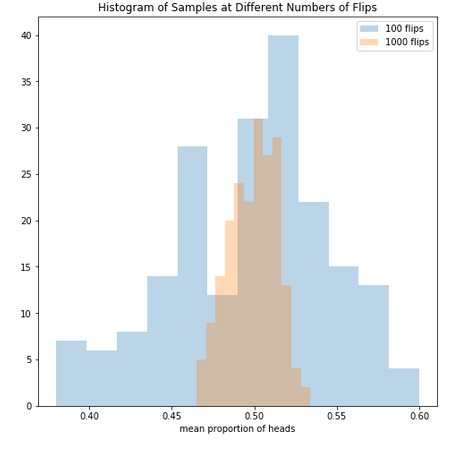
\includegraphics{./HW0Plot2.png}

\textbf{3.3}. Calculate the mean and variance of the results in the each
of the variables \texttt{proportions\_at\_n\_flips\_100} and
\texttt{proportions\_at\_n\_flips\_1000} generated in 3.2.

\textbf{3.4}. Based upon the plots what would be your guess of what type
of distribution is represented by histograms in 3.2? Explain the factors
that influenced your choice. \textgreater{} A. Gamma Distribution
\textgreater{} \textgreater{} B. Beta Distribution \textgreater{}
\textgreater{} C. Gaussian

\textbf{3.5}. Let's just assume for arguments sake that the answer to
3.4 is \textbf{C. Gaussian}. Plot a \textbf{normed histogram} of your
results \texttt{proportions\_at\_n\_flips\_1000} overlayed with your
selection for the appropriate gaussian distribution to represent the
experiment of flipping a coin 1000 times. (\textbf{Hint: What parameters
should you use for your Gaussian?})

    \textbf{3.1}

    \begin{Verbatim}[commandchars=\\\{\}]
{\color{incolor}In [{\color{incolor}14}]:} \PY{c+c1}{\PYZsh{} your code here}
\end{Verbatim}


    \textbf{3.2}

    \begin{Verbatim}[commandchars=\\\{\}]
{\color{incolor}In [{\color{incolor}15}]:} \PY{c+c1}{\PYZsh{} your code here}
\end{Verbatim}


    \begin{Verbatim}[commandchars=\\\{\}]
{\color{incolor}In [{\color{incolor}16}]:} \PY{c+c1}{\PYZsh{} code for your plot here}
\end{Verbatim}


    \textbf{3.3}

    \begin{Verbatim}[commandchars=\\\{\}]
{\color{incolor}In [{\color{incolor}21}]:} \PY{c+c1}{\PYZsh{} your code here}
\end{Verbatim}


    \textbf{3.4}

    ** Your choice and explanation here **

    \textbf{3.5}

    \begin{Verbatim}[commandchars=\\\{\}]
{\color{incolor}In [{\color{incolor}21}]:} \PY{c+c1}{\PYZsh{} your code here}
\end{Verbatim}


    \subsection{Working With Distributions in
Numpy/Scipy}\label{working-with-distributions-in-numpyscipy}

Earlier in this problem set we've been introduced to the Bernoulli "aka
coin-flip" distribution and worked with it indirectly by using
np.random.choice to make a random selection between two elements 'H' and
'T'. Let's see if we can create comparable results by taking advantage
of the machinery for working with other probability distributions in
python using numpy and scipy.

    \#\#\#

Question 4: My Normal Binomial

Let's use our coin-flipping machinery to do some experimentation with
the binomial distribution. The binomial distribution, often represented
by \(k \sim Binomial(n, p)\) is often discribed the number of successes
in \texttt{n} Bernoulli trials with each trial having a probability of
success \texttt{p}. In other words, if you flip a coin \texttt{n} times,
and each coin-flip has a probability \texttt{p} of landing heads, then
the number of heads you observe is a sample from a binomial
distribution.

\textbf{4.1}. Sample the binomial distribution with \(p = 0.5\) using
coin flips by writing a function \texttt{sample\_binomial1} which takes
in integer parameters \texttt{n} and \texttt{size}. The output of
\texttt{sample\_binomial1} should be a list of length \texttt{size}
observations with each observation being the outcome of flipping a coin
\texttt{n} times and counting the number of heads. By default
\texttt{size} should be 1. Your code should take advantage of the
\texttt{throw\_a\_coin} function we defined above.

\textbf{4.2}. Sample the binomial distribution directly using
scipy.stats.binom.rvs by writing another function
\texttt{sample\_binomial2} that takes in integer parameters \texttt{n}
and \texttt{size} as well as a float \texttt{p} parameter \texttt{p}
where \(p \in [0 \ldots 1]\). The output of \texttt{sample\_binomial2}
should be a list of length \texttt{size} observations with each
observation a sample of \(Binomial(n, p)\) (taking advantage of
scipy.stats.binom). By default \texttt{size} should be 1 and \texttt{p}
should be 0.5.

\textbf{4.3}. Run sample\_binomial1 with 25 and 200 as values of the
\texttt{n} and \texttt{size} parameters respectively and store the
result in \texttt{binomial\_trials1}. Run sample\_binomial2 with 25, 200
and 0.5 as values of the \texttt{n}, \texttt{size} and \texttt{p}
parameters respectively and store the results in
\texttt{binomial\_trials2}. Plot normed histograms of
\texttt{binomial\_trials1} and \texttt{binomial\_trials2}. On both
histograms, overlay a plot of the pdf of \(Binomial(n=25, p=0.5)\)

\textbf{4.4}. How do the plots in 4.3 compare?

\textbf{4.5}. Find the mean and variance of \texttt{binomial\_trials1}.
How do they compare to the true mean and varaince of a
\(Binomial(n=25, p=0.5)\) distribution?

    \paragraph{Answers}\label{answers}

    \textbf{4.1}

    \begin{Verbatim}[commandchars=\\\{\}]
{\color{incolor}In [{\color{incolor}17}]:} \PY{c+c1}{\PYZsh{} your code here}
\end{Verbatim}


    \textbf{4.2}

    \begin{Verbatim}[commandchars=\\\{\}]
{\color{incolor}In [{\color{incolor}18}]:} \PY{c+c1}{\PYZsh{} your code}
\end{Verbatim}


    \textbf{4.3}

    \begin{Verbatim}[commandchars=\\\{\}]
{\color{incolor}In [{\color{incolor}20}]:} \PY{c+c1}{\PYZsh{} your code here}
\end{Verbatim}


    \textbf{4.4}

    ** Your explanation here **

    \textbf{4.5}

    \begin{Verbatim}[commandchars=\\\{\}]
{\color{incolor}In [{\color{incolor} }]:} \PY{c+c1}{\PYZsh{} your code here }
\end{Verbatim}


    ** Your explanation here **

    \subsection{Testing Your Python Code}\label{testing-your-python-code}

    In the following section we're going to do a brief introduction to unit
testing. We do so not only because unit testing has become an
increasingly important part of of the methodology of good software
practices, but also because we plan on using unit tests as part of our
own CS109 grading practices as a way of increasing rigor and
repeatability decreasing complexity and manual workload in our
evaluations of your code. We'll provide an example unit test at the end
of this section.

\subsubsection{Introduction to unit
testing}\label{introduction-to-unit-testing}

    \begin{Verbatim}[commandchars=\\\{\}]
{\color{incolor}In [{\color{incolor}45}]:} \PY{k+kn}{import} \PY{n+nn}{ipytest}
\end{Verbatim}


    \textbf{\emph{Unit testing}} is one of the most important software
testing methodologies. Wikipedia describes unit testing as "a software
testing method by which individual units of source code, sets of one or
more computer program modules together with associated control data,
usage procedures, and operating procedures, are tested to determine
whether they are fit for use."

There are many different python libraries that support software testing
in general and unit testing in particular. PyTest is one of the most
widely used and well-liked libraries for this purpose. We've chosen to
adopt PyTest (and ipytest which allows pytest to be used in ipython
notebooks) for our testing needs and we'll do a very brief introduction
to Pytest here so that you can become familiar with it too.

If you recall the function that we provided you above
\texttt{throw\_a\_coin}, which we'll reproduce here for convenience, it
took a number and returned that many "coin tosses". We'll start by
seeing what happens when we give it different sizes of \(N\). If we give
\(N=0\), we should get an empty array of "experiments".

    \begin{Verbatim}[commandchars=\\\{\}]
{\color{incolor}In [{\color{incolor}39}]:} \PY{k}{def} \PY{n+nf}{throw\PYZus{}a\PYZus{}coin}\PY{p}{(}\PY{n}{N}\PY{p}{)}\PY{p}{:}
             \PY{k}{return} \PY{n}{np}\PY{o}{.}\PY{n}{random}\PY{o}{.}\PY{n}{choice}\PY{p}{(}\PY{p}{[}\PY{l+s+s1}{\PYZsq{}}\PY{l+s+s1}{H}\PY{l+s+s1}{\PYZsq{}}\PY{p}{,}\PY{l+s+s1}{\PYZsq{}}\PY{l+s+s1}{T}\PY{l+s+s1}{\PYZsq{}}\PY{p}{]}\PY{p}{,} \PY{n}{size}\PY{o}{=}\PY{n}{N}\PY{p}{)}
\end{Verbatim}


    \begin{Verbatim}[commandchars=\\\{\}]
{\color{incolor}In [{\color{incolor}46}]:} \PY{n}{throw\PYZus{}a\PYZus{}coin}\PY{p}{(}\PY{l+m+mi}{0}\PY{p}{)}
\end{Verbatim}


\begin{Verbatim}[commandchars=\\\{\}]
{\color{outcolor}Out[{\color{outcolor}46}]:} array([], dtype='<U1')
\end{Verbatim}
            
    Great! If we give it positive values of \(N\) we should get that number
of 'H's and 'T's.

    \begin{Verbatim}[commandchars=\\\{\}]
{\color{incolor}In [{\color{incolor}47}]:} \PY{n}{throw\PYZus{}a\PYZus{}coin}\PY{p}{(}\PY{l+m+mi}{5}\PY{p}{)}
\end{Verbatim}


\begin{Verbatim}[commandchars=\\\{\}]
{\color{outcolor}Out[{\color{outcolor}47}]:} array(['H', 'H', 'T', 'T', 'T'], dtype='<U1')
\end{Verbatim}
            
    \begin{Verbatim}[commandchars=\\\{\}]
{\color{incolor}In [{\color{incolor}48}]:} \PY{n}{throw\PYZus{}a\PYZus{}coin}\PY{p}{(}\PY{l+m+mi}{8}\PY{p}{)}
\end{Verbatim}


\begin{Verbatim}[commandchars=\\\{\}]
{\color{outcolor}Out[{\color{outcolor}48}]:} array(['T', 'T', 'H', 'H', 'H', 'T', 'T', 'T'], dtype='<U1')
\end{Verbatim}
            
    Exactly what we expected!

What happens if the input isn't a positive integer though?

    \begin{Verbatim}[commandchars=\\\{\}]
{\color{incolor}In [{\color{incolor}43}]:} \PY{n}{throw\PYZus{}a\PYZus{}coin}\PY{p}{(}\PY{l+m+mf}{4.5}\PY{p}{)}
\end{Verbatim}


    \begin{Verbatim}[commandchars=\\\{\}]

        ---------------------------------------------------------------------------

        TypeError                                 Traceback (most recent call last)

        <ipython-input-43-7a98054470df> in <module>()
    ----> 1 throw\_a\_coin(4.5)
    

        <ipython-input-39-9b62022d816e> in throw\_a\_coin(N)
          1 def throw\_a\_coin(N):
    ----> 2     return np.random.choice(['H','T'], size=N)
    

        mtrand.pyx in mtrand.RandomState.choice()


        mtrand.pyx in mtrand.RandomState.randint()


        mtrand.pyx in mtrand.RandomState.randint()


        randint\_helpers.pxi in mtrand.\_rand\_int64()


        TypeError: 'float' object cannot be interpreted as an integer

    \end{Verbatim}

    or

    \begin{Verbatim}[commandchars=\\\{\}]
{\color{incolor}In [{\color{incolor}44}]:} \PY{n}{throw\PYZus{}a\PYZus{}coin}\PY{p}{(}\PY{o}{\PYZhy{}}\PY{l+m+mi}{4}\PY{p}{)}
\end{Verbatim}


    \begin{Verbatim}[commandchars=\\\{\}]

        ---------------------------------------------------------------------------

        ValueError                                Traceback (most recent call last)

        <ipython-input-44-8560c28a4e91> in <module>()
    ----> 1 throw\_a\_coin(-4)
    

        <ipython-input-39-9b62022d816e> in throw\_a\_coin(N)
          1 def throw\_a\_coin(N):
    ----> 2     return np.random.choice(['H','T'], size=N)
    

        mtrand.pyx in mtrand.RandomState.choice()


        mtrand.pyx in mtrand.RandomState.randint()


        mtrand.pyx in mtrand.RandomState.randint()


        randint\_helpers.pxi in mtrand.\_rand\_int64()


        ValueError: negative dimensions are not allowed

    \end{Verbatim}

    It looks like for both real numbers and negative numbers, we get two
kinds of errors a \texttt{TypeError} and a \texttt{ValueError}. We just
engaged in one of the most rudimentary forms of testing, trial and
error. We can use pytest to automate this process by writing some
functions that will automatically (and potentially repeatedly) test
individual units of our code methodology. These are called
\textbf{\emph{unit tests}}.

Before we write our tests, let's consider what we would think of as the
approrpriate behavior for \texttt{throw\_a\_coin} under the conditions
we considered above. If \texttt{throw\_a\_coin} receives positive
integer input, we want it to behave exactly as it currently does -\/-
returning an output consisting of a list of characters 'H' or 'T' with
the length of the list equal to the positive integer input. For a
positive floating point input, we want \texttt{throw\_a\_coin\_properly}
to treat the input as if it were rounded down to the nearest integer
thus returning a list of 'H' or 'T' integers whose length is the same as
the input rounded down to the next highest integer. For a any negative
number input or an input of 0, we want \texttt{throw\_a\_coin\_properly}
to return an empty list.

    We create pytest tests by writing functions that start or end with
"test". We'll use the \textbf{convention} that our tests will start with
"test".

We begin the code cell with ipytest's clean\_tests function as a way to
clear out the results of previous tests starting with
"test\_throw\_a\_coin" (the * is the standard wild card charater here).

    \begin{Verbatim}[commandchars=\\\{\}]
{\color{incolor}In [{\color{incolor} }]:} \PY{c+c1}{\PYZsh{}\PYZsh{} the * after test\PYZus{}throw\PYZus{}a\PYZus{}coin tells this code cell to clean out the results}
        \PY{c+c1}{\PYZsh{}\PYZsh{} of all tests starting with test\PYZus{}throw\PYZus{}a\PYZus{}coin}
        \PY{n}{ipytest}\PY{o}{.}\PY{n}{clean\PYZus{}tests}\PY{p}{(}\PY{l+s+s2}{\PYZdq{}}\PY{l+s+s2}{test\PYZus{}throw\PYZus{}a\PYZus{}coin*}\PY{l+s+s2}{\PYZdq{}}\PY{p}{)}
        
        \PY{c+c1}{\PYZsh{}\PYZsh{} run throw\PYZus{}a\PYZus{}coin with a variety of positive integer inputs (all numbers between 1 and 20) and}
        \PY{c+c1}{\PYZsh{}\PYZsh{} verify that the length of the output list (e.g [\PYZsq{}H\PYZsq{}, \PYZsq{}H\PYZsq{}, \PYZsq{}T\PYZsq{}, \PYZsq{}H\PYZsq{}, \PYZsq{}T\PYZsq{}]) matches the input integer}
        \PY{k}{def} \PY{n+nf}{test\PYZus{}throw\PYZus{}a\PYZus{}coin\PYZus{}length\PYZus{}positive}\PY{p}{(}\PY{p}{)}\PY{p}{:}
            \PY{k}{for} \PY{n}{n} \PY{o+ow}{in} \PY{n+nb}{range}\PY{p}{(}\PY{l+m+mi}{1}\PY{p}{,}\PY{l+m+mi}{20}\PY{p}{)}\PY{p}{:}
                \PY{k}{assert} \PY{n+nb}{len}\PY{p}{(}\PY{n}{throw\PYZus{}a\PYZus{}coin}\PY{p}{(}\PY{n}{n}\PY{p}{)}\PY{p}{)} \PY{o}{==} \PY{n}{n}
        
        \PY{c+c1}{\PYZsh{}\PYZsh{} verify that throw\PYZus{}a\PYZus{}coin produces an empty list (i.e. a list of length 0) if provide with an input}
        \PY{c+c1}{\PYZsh{}\PYZsh{} of 0}
        \PY{k}{def} \PY{n+nf}{test\PYZus{}throw\PYZus{}a\PYZus{}coin\PYZus{}length\PYZus{}zero}\PY{p}{(}\PY{p}{)}\PY{p}{:}
            \PY{c+c1}{\PYZsh{}\PYZsh{} should be the empty array}
            \PY{k}{assert} \PY{n+nb}{len}\PY{p}{(}\PY{n}{throw\PYZus{}a\PYZus{}coin}\PY{p}{(}\PY{l+m+mi}{0}\PY{p}{)}\PY{p}{)} \PY{o}{==} \PY{l+m+mi}{0}
            
        
        \PY{c+c1}{\PYZsh{}\PYZsh{} verify that given a positive floating point input (i.e. 4.34344298547201), throw\PYZus{}a\PYZus{}coin produces a list of}
        \PY{c+c1}{\PYZsh{}\PYZsh{} coin flips of length equal to highest integer less than the input}
        \PY{k}{def} \PY{n+nf}{test\PYZus{}throw\PYZus{}a\PYZus{}coin\PYZus{}float}\PY{p}{(}\PY{p}{)}\PY{p}{:}
            \PY{k}{for} \PY{n}{n} \PY{o+ow}{in} \PY{n}{np}\PY{o}{.}\PY{n}{random}\PY{o}{.}\PY{n}{exponential}\PY{p}{(}\PY{l+m+mi}{7}\PY{p}{,} \PY{n}{size}\PY{o}{=}\PY{l+m+mi}{5}\PY{p}{)}\PY{p}{:}
                \PY{k}{assert} \PY{n+nb}{len}\PY{p}{(}\PY{n}{throw\PYZus{}a\PYZus{}coin}\PY{p}{(}\PY{n}{n}\PY{p}{)}\PY{p}{)} \PY{o}{==} \PY{n}{np}\PY{o}{.}\PY{n}{floor}\PY{p}{(}\PY{n}{n}\PY{p}{)}
                
        
        \PY{c+c1}{\PYZsh{}\PYZsh{} verify that given any negative input (e.g. \PYZhy{}323.4), throw\PYZus{}a\PYZus{}coin produces an empty}
        \PY{k}{def} \PY{n+nf}{test\PYZus{}throw\PYZus{}a\PYZus{}coin\PYZus{}negative}\PY{p}{(}\PY{p}{)}\PY{p}{:}
            \PY{k}{for} \PY{n}{n} \PY{o+ow}{in} \PY{n+nb}{range}\PY{p}{(}\PY{o}{\PYZhy{}}\PY{l+m+mi}{7}\PY{p}{,} \PY{l+m+mi}{0}\PY{p}{)}\PY{p}{:}
                \PY{k}{assert} \PY{n+nb}{len}\PY{p}{(}\PY{n}{throw\PYZus{}a\PYZus{}coin}\PY{p}{(}\PY{n}{n}\PY{p}{)}\PY{p}{)} \PY{o}{==} \PY{l+m+mi}{0}
        
                
        \PY{n}{ipytest}\PY{o}{.}\PY{n}{run\PYZus{}tests}\PY{p}{(}\PY{p}{)}
\end{Verbatim}


    As you see, we were able to use pytest (and ipytest which allows us to
run pytest tests in our ipython notebooks) to automate the tests that we
constructed manually before and get the same errors and successes. Now
time to fix our code and write our own test!

    \#\#\#

Question 5: You Better Test Yourself before You Wreck Yourself!

Now it's time to fix \texttt{throw\_a\_coin} so that it passes the tests
we've written above as well as add our own test to the mix!

\textbf{5.1}. Write a new function called
\texttt{throw\_a\_coin\_properly} that will pass the tests that we saw
above. For your convenience we'll provide a new jupyter notebook cell
with the tests rewritten for the new function. All the tests should
pass. For a positive floating point input, we want
\texttt{throw\_a\_coin\_properly} to treat the input as if it were
rounded down to the nearest integer. For a any negative number input, we
want \texttt{throw\_a\_coin\_properly} to treat the input as if it were
0.

\textbf{5.2}. Write a new test for \texttt{throw\_a\_coin\_properly}
that verifies that all the elements of the resultant arrays are 'H' or
'T'.

    \paragraph{Answers}\label{answers}

    \textbf{5.1}

    \begin{Verbatim}[commandchars=\\\{\}]
{\color{incolor}In [{\color{incolor}21}]:} \PY{k}{def} \PY{n+nf}{throw\PYZus{}a\PYZus{}coin\PYZus{}properly}\PY{p}{(}\PY{n}{n\PYZus{}trials}\PY{p}{)}\PY{p}{:}
             
             \PY{c+c1}{\PYZsh{} your code here}
             
\end{Verbatim}


    \begin{Verbatim}[commandchars=\\\{\}]
{\color{incolor}In [{\color{incolor} }]:} \PY{n}{ipytest}\PY{o}{.}\PY{n}{clean\PYZus{}tests}\PY{p}{(}\PY{l+s+s2}{\PYZdq{}}\PY{l+s+s2}{test\PYZus{}throw\PYZus{}a\PYZus{}coin*}\PY{l+s+s2}{\PYZdq{}}\PY{p}{)}
        
        \PY{k}{def} \PY{n+nf}{test\PYZus{}throw\PYZus{}a\PYZus{}coin\PYZus{}properly\PYZus{}length\PYZus{}positive}\PY{p}{(}\PY{p}{)}\PY{p}{:}
            \PY{k}{for} \PY{n}{n} \PY{o+ow}{in} \PY{n+nb}{range}\PY{p}{(}\PY{l+m+mi}{1}\PY{p}{,}\PY{l+m+mi}{20}\PY{p}{)}\PY{p}{:}
                \PY{k}{assert} \PY{n+nb}{len}\PY{p}{(}\PY{n}{throw\PYZus{}a\PYZus{}coin\PYZus{}properly}\PY{p}{(}\PY{n}{n}\PY{p}{)}\PY{p}{)} \PY{o}{==} \PY{n}{n}
                
        
        \PY{k}{def} \PY{n+nf}{test\PYZus{}throw\PYZus{}a\PYZus{}coin\PYZus{}properly\PYZus{}length\PYZus{}zero}\PY{p}{(}\PY{p}{)}\PY{p}{:}
            \PY{c+c1}{\PYZsh{}\PYZsh{} should be the empty array}
            \PY{k}{assert} \PY{n+nb}{len}\PY{p}{(}\PY{n}{throw\PYZus{}a\PYZus{}coin\PYZus{}properly}\PY{p}{(}\PY{l+m+mi}{0}\PY{p}{)}\PY{p}{)} \PY{o}{==} \PY{l+m+mi}{0}
            
        
        \PY{k}{def} \PY{n+nf}{test\PYZus{}throw\PYZus{}a\PYZus{}coin\PYZus{}properly\PYZus{}float}\PY{p}{(}\PY{p}{)}\PY{p}{:}
            
            \PY{k}{for} \PY{n}{n} \PY{o+ow}{in} \PY{n}{np}\PY{o}{.}\PY{n}{random}\PY{o}{.}\PY{n}{exponential}\PY{p}{(}\PY{l+m+mi}{7}\PY{p}{,} \PY{n}{size}\PY{o}{=}\PY{l+m+mi}{5}\PY{p}{)}\PY{p}{:}
                \PY{k}{assert} \PY{n+nb}{len}\PY{p}{(}\PY{n}{throw\PYZus{}a\PYZus{}coin\PYZus{}properly}\PY{p}{(}\PY{n}{n}\PY{p}{)}\PY{p}{)} \PY{o}{==} \PY{n}{np}\PY{o}{.}\PY{n}{floor}\PY{p}{(}\PY{n}{n}\PY{p}{)}
                
        
        \PY{k}{def} \PY{n+nf}{test\PYZus{}throw\PYZus{}a\PYZus{}coin\PYZus{}properly\PYZus{}negative}\PY{p}{(}\PY{p}{)}\PY{p}{:}
            
            \PY{k}{for} \PY{n}{n} \PY{o+ow}{in} \PY{n+nb}{range}\PY{p}{(}\PY{o}{\PYZhy{}}\PY{l+m+mi}{7}\PY{p}{,} \PY{l+m+mi}{0}\PY{p}{)}\PY{p}{:}
                \PY{k}{assert} \PY{n+nb}{len}\PY{p}{(}\PY{n}{throw\PYZus{}a\PYZus{}coin\PYZus{}properly}\PY{p}{(}\PY{n}{n}\PY{p}{)}\PY{p}{)} \PY{o}{==} \PY{l+m+mi}{0}
        
                
        \PY{n}{ipytest}\PY{o}{.}\PY{n}{run\PYZus{}tests}\PY{p}{(}\PY{p}{)}
\end{Verbatim}


    \textbf{5.2}

    \begin{Verbatim}[commandchars=\\\{\}]
{\color{incolor}In [{\color{incolor} }]:} \PY{n}{ipytest}\PY{o}{.}\PY{n}{clean\PYZus{}tests}\PY{p}{(}\PY{l+s+s2}{\PYZdq{}}\PY{l+s+s2}{test\PYZus{}throw\PYZus{}a\PYZus{}coin*}\PY{l+s+s2}{\PYZdq{}}\PY{p}{)}
        
        \PY{c+c1}{\PYZsh{}\PYZsh{} write a test that verifies you don\PYZsq{}t have any other elements except H\PYZsq{}s and T\PYZsq{}s}
        \PY{k}{def} \PY{n+nf}{test\PYZus{}throw\PYZus{}a\PYZus{}coin\PYZus{}properly\PYZus{}verify\PYZus{}H\PYZus{}T}\PY{p}{(}\PY{p}{)}\PY{p}{:}
            
            \PY{c+c1}{\PYZsh{} your code here }
                
                
        \PY{n}{ipytest}\PY{o}{.}\PY{n}{run\PYZus{}tests}\PY{p}{(}\PY{p}{)}
\end{Verbatim}


    \begin{Verbatim}[commandchars=\\\{\}]
{\color{incolor}In [{\color{incolor}66}]:} 
\end{Verbatim}


\begin{Verbatim}[commandchars=\\\{\}]
{\color{outcolor}Out[{\color{outcolor}66}]:} <IPython.core.display.HTML object>
\end{Verbatim}
            

    % Add a bibliography block to the postdoc
    
    
    
    \end{document}
